\section{Introduction}
\label{s:lab2-introduction}
Active enumeration is when a user programmatically gather informations on a system through
the use of a set of predefined commands.The most common set of informations that is
usually gathered through enumeration are DNS, IPs, ports, and services.

\section{Code}
\label{s:lab2-code}
\begin{figure}[H]
  \centering
  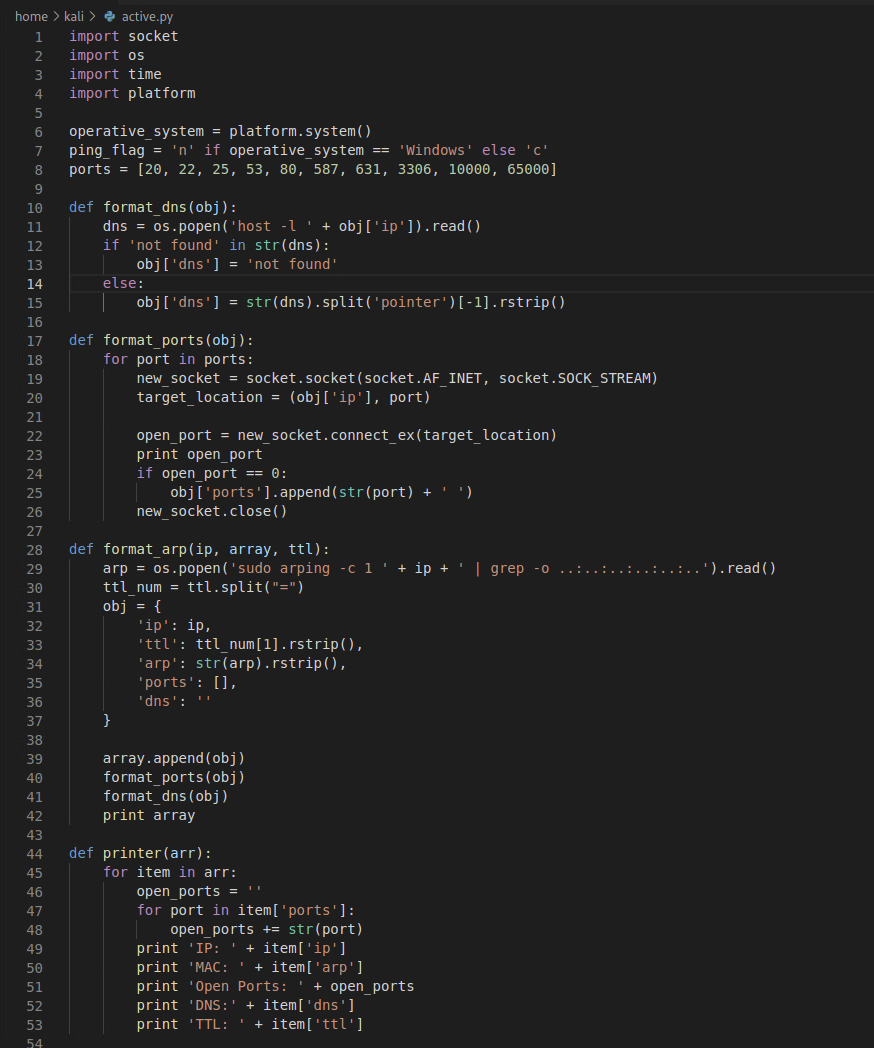
\includegraphics[width=0.6\textwidth]{figures/code/functions}
  \caption{Functions of the Program}
  \label{f:functions}
\end{figure}

\begin{figure}[H]
  \centering
  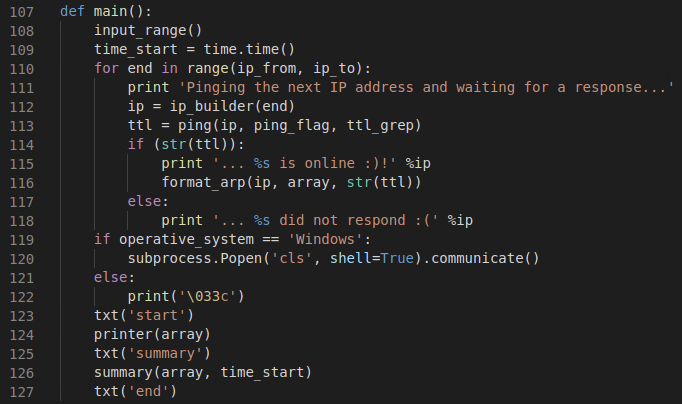
\includegraphics[width=0.6\textwidth]{figures/code/main}
  \caption{Main of the Program}
  \label{f:main}
\end{figure}

\begin{figure}[H]
  \centering
  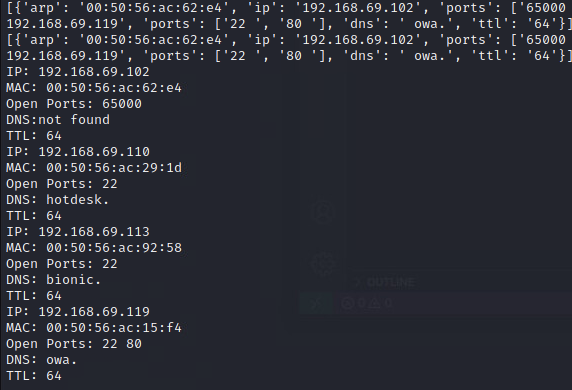
\includegraphics[width=0.6\textwidth]{figures/program-result}
  \caption{program-result}
  \label{f:program-result}
\end{figure}
